%    \samsection{0. bird's eye view}
%~~~~~~~~~~~~~~~~~~~~~~~~~~~~~~~~~~~~~~~~~~~~~~~~~~~~~~~~~~~~~~~~~~~~~~~~~~~~~~
%~~~~~~~~~~~~~  1.0. kinds of learning  ~~~~~~~~~~~~~~~~~~~~~~~~~~~~~~~~~~~~~~~

      \sampassage{kinds of learning}
        How do we communicate patterns of desired behavior?  We can teach:
        \begin{description}
          \item[\textbf{by instruction}:  ]  ``to tell whether a mushroom is poisonous, first look at its gills...''
          \item[\textbf{by example}:      ]  ``here are six poisonous fungi; here, six safe ones.  see a pattern?''
          \item[\textbf{by reinforcement}:]  ``eat foraged mushrooms for a month; learn from getting sick.''
        \end{description}
        %
        \marginnote{%
          \attn{Exercise:} What's a thing you know now but not last month?
          What kinds of signal taught you?
        }
        Machine learning is the art of programming computers to learn from such
        sources.  We'll focus on the most important case: \textbf{learning from
        examples}.\bcirc\marginnote{%
          \blarr In part E, we'll see that learning by example is key to
          the other modes of learning.
        }

%~~~~~~~~~~~~~~~~~~~~~~~~~~~~~~~~~~~~~~~~~~~~~~~~~~~~~~~~~~~~~~~~~~~~~~~~~~~~~~
%~~~~~~~~~~~~~  1.1. from examples to predictions  ~~~~~~~~~~~~~~~~~~~~~~~~~~~~

      \sampassage{from examples to predictions}
        For us, a pattern of desired behavior is a function that for each given
        situation/prompt returns a favorable action/answer.
        %
        Our goal is to write a program that, from a list of $N$ examples of
        prompts and matching answers, determines an underlying pattern.  We
        consider our program a success if this pattern accurately predicts
        answers corresponding to new, unseen prompts.
        %
        We often define our program as a search, over some set $\hH$ of
        candidate patterns, to minimize some notion of ``discrepancy from the
        example data''.

        \begin{figure}[h]
          \vspace{-0.5cm}
          \par\noindent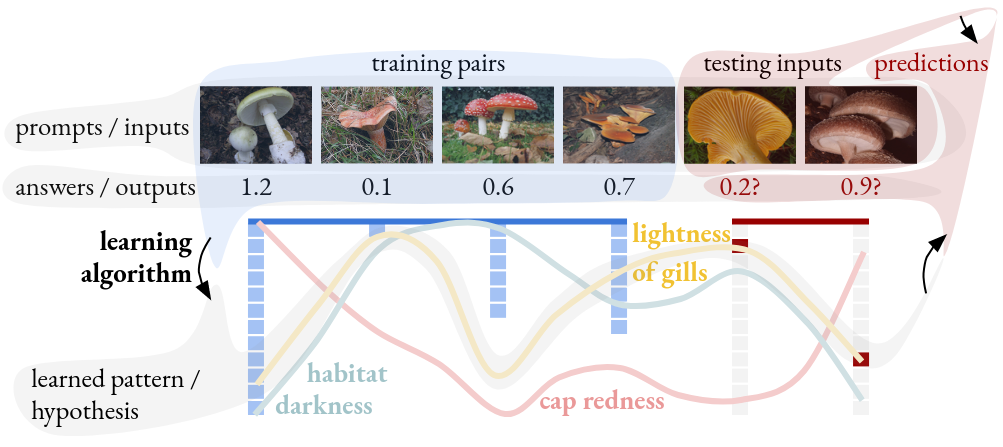
\includegraphics[width=\textwidth]{figures/supervised}\\
          \caption{%
            A program that learns to predict mushrooms' poison levels:
            %
            first takes a list of labeled mushrooms as input (blue blob);
            searches
            through candidate patterns (here, the wiggly curves labeled
            \texttt{lightness of gills}, \texttt{habitat darkness}, and
            \texttt{cap redness}); and returns the pattern that best fits the
            examples.
            %
            Evaluating this pattern on new mushrooms, we predict their poison
            levels (red blob).
            %
            \par Three arrows show how
            training examples induce a learned pattern, which,
            together with testing prompts, induces predictions.
            %
            Part of specifying the learning program is specifying the set of candidate patterns to consider.
          }
          \vspace{-1.0cm}
        \end{figure}

        To save ink, say that $\xX$ is the set of possible prompts; $\yY$, of
        possible answers.\bcirc\marginnote{%
          \blarr If we like, we can now summarize the data flow in symbols.  A
          pattern is a function of type $\xX\to\yY$.  And we can model the
          examples from which our program learns as a list of type $(\xX\times
          \yY)^N$.  Then a program that learns from examples has type:
          $$
            \lL : (\xX\times \yY)^N \to (\xX\to \yY)
          $$
          Once we allow uncertainty by letting patterns map to \emph{probability
          distributions} over answers, the type will change to:
          $$
            \lL : (\xX\times \yY)^N \to (\xX\to \text{DistributionsOn}(\yY))
          $$
        }
        In the mushrooms example, $\xX$ contains all
        conceivable mushrooms and $\yY$ contains all conceivable poison
        levels (perhaps all the non-negative real numbers).

%~~~~~~~~~~~~~~~~~~~~~~~~~~~~~~~~~~~~~~~~~~~~~~~~~~~~~~~~~~~~~~~~~~~~~~~~~~~~~~
%~~~~~~~~~~~~~  1.2. supervised learning  ~~~~~~~~~~~~~~~~~~~~~~~~~~~~~~~~~~~~~

      \sampassage{supervised learning}
        We'll soon allow uncertainty by letting patterns map to
        \emph{probability measures} over answers.
        %
        Even if $|X|=1$ --- say, $X=\{$``produce a beautiful melody''$\}$ ---
        we may seek to learn the complicated distribution over answers,
        e.g.\ to generate a diversity of apt answers.
        %
        So-called \textbf{unsupervised learning} thus concerns output
        structure.  By contrast, \textbf{supervised learning} (our main subject), concerns the input-output
        relation; it's interesting when there are many possible
        prompts.
        %


